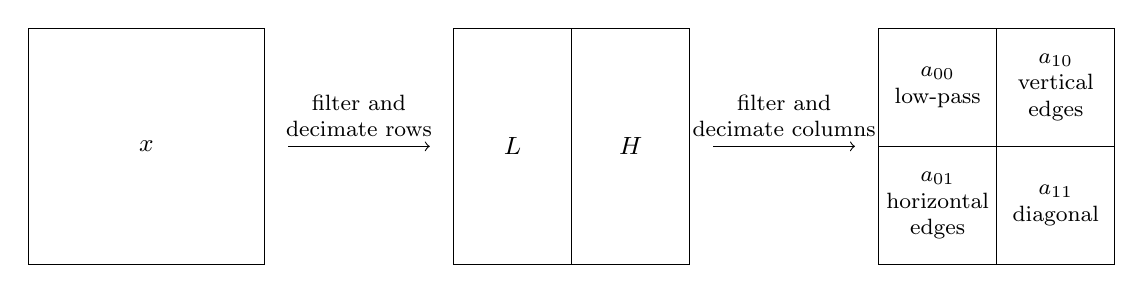
\begin{tikzpicture}[x=1cm,y=-1cm,font=\small]
  % input
  \draw (0,0) rectangle (3,3);
  \node at (1.5,1.5) {$x$};
  \draw[->] (3.3,1.5) -- node[above,font=\footnotesize,align=center] {filter and\\decimate rows} (5.1,1.5);
  % after rows
  \draw (5.4,0) rectangle (8.4,3);
  \draw (6.9,0) -- (6.9,3);
  \node at (6.15,1.5) {$L$};
  \node at (7.65,1.5) {$H$};
  \draw[->] (8.7,1.5) -- node[above,font=\footnotesize,align=center] {filter and\\decimate columns} (10.5,1.5);
  % after columns
  \draw (10.8,0) rectangle (13.8,3);
  \draw (12.3,0) -- (12.3,3) (10.8,1.5) -- (13.8,1.5);
  \node[align=center,font=\footnotesize] at (11.55,0.75) {$a_{00}$\\low-pass};
  \node[align=center,font=\footnotesize] at (13.05,0.75) {$a_{10}$\\vertical\\edges};
  \node[align=center,font=\footnotesize] at (11.55,2.25) {$a_{01}$\\horizontal\\edges};
  \node[align=center,font=\footnotesize] at (13.05,2.25) {$a_{11}$\\diagonal};
\end{tikzpicture}
